\section{Smooth Obstacles}
The step-avoiding route shown in Figure 2 is only one example among a family of routes with equal cost. A smoothly-varying obstacle breaks this degeneracy and determines a finite number of optimal paths.

By smoothly-varying, we mean that the derivative of $f$ is defined everywhere. One such example, commonly used to model obstacles, is the Gaussian.

\begin{equation}
f(x, y) = A \exp\left(-\displaystyle\frac{x^2+y^2}{2\sigma^2}\right)
\end{equation}

The Gaussian is radially symmetric, and it decreases monotonically from its center. Both properties are sensible ones for modeling a simple obstacle.

Restricted rook-like motion in our 4-connected space, we can immediately see that all movements take the shape of a bracket: a path from $(-n,0)$ to $(-n, \yhat)$ to $(n, \yhat)$ to $(n,0)$ for some $\yhat$. (Or, equivalently, the mirror image in $y \rightarrow -y$.) If any traverse steps are taken, they should always be taken at the edge of the space, as far from the origin as possible.

\begin{figure}
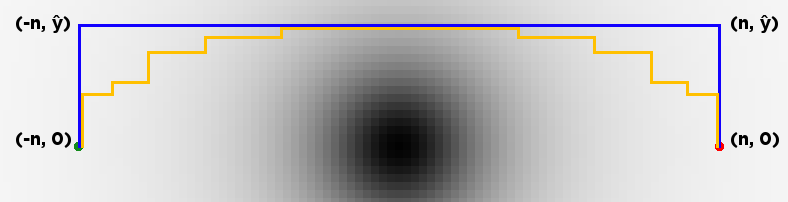
\includegraphics[width=\columnwidth]{graphix/bracket.png}
\caption{The Bracket Shape}
\label{fig:bracket}
\end{figure}